\clearpage
\subsection{Restricted deployment and fresh confirmation}
The broad test exposes incomplete equation filters in the new vacuum
profiles. Their native fallback retains exact results and adds cost.
We therefore fix a restricted deployment using the same trained tree.
It enables the equation filter at $\tau=0.001$ for the recorded
21-target sunrise batches and retains native equation choices for
other topologies and target sets. The broader test supplies development
evidence for this deployment revision.

Each supported batch contains the top-sector scalar integral and its
one-dot and one-numerator variants, together with the corresponding
integrals in the three two-propagator sectors. This gives 21 targets
whose index vectors are fixed in the deployment definition.
We reserve six additional mass and momentum profiles before running
their reductions. None of these profiles occurs in the preceding
training, validation or broad-test sets. Their squared masses and
external invariant are fixed rational numbers, while $d$ remains symbolic.
The tree, threshold, target domain and new profile definitions are
fixed before this confirmation begins.

Nine alternating repetitions compare the learned filter, native choices
and the previously selected distance control in each profile. These
162 complete workflows use the same timing and exact-check rules
as the preceding test, including every failed attempt.

The learned filter has a complete-time ratio of 0.994, with descriptive interval $[0.991,0.997]$ and an equation-preparation ratio of 0.785, with descriptive interval $[0.776,0.794]$. Its generated-equation ratio is 0.414, and its selected-equation ratio is 1.000. The distance control has a complete-time ratio of 1.003, with descriptive interval $[1.000,1.006]$.

The complete-time interval remains below one for these six profiles, supporting a measured gain within the restricted domain.

A further 36 workflows compare the existing seed and row policies with the configuration that also includes the equation filter. Adding the third model gives a complete-time ratio of 1.317, with descriptive interval $[1.296,1.337]$ and a preparation ratio of 1.151, with descriptive interval $[1.136,1.168]$ to the two-model configuration. This comparison uses three repetitions in each of the six profiles.

All 162 main workflows, 36 composition workflows and six basis-only applications pass the independent exact audit, which checks 7,582 coefficient pairs. The 204 workflows include 54 failed attempts. The six applications receive the prescribed masters without reference target coefficients, and their outputs pass coefficient comparisons after execution.

Native median complete times range from 0.692 to 0.709 seconds in these six profiles. The geometric mean preparation fraction of native complete time is 3.29\%. This small fraction explains why the reduction in preparation time produces a smaller change in complete time. The main confirmation has zero failed attempts; all 54 failed attempts in its extended audit arise in the composition comparisons.

\begin{figure}[htbp]
 \centering
 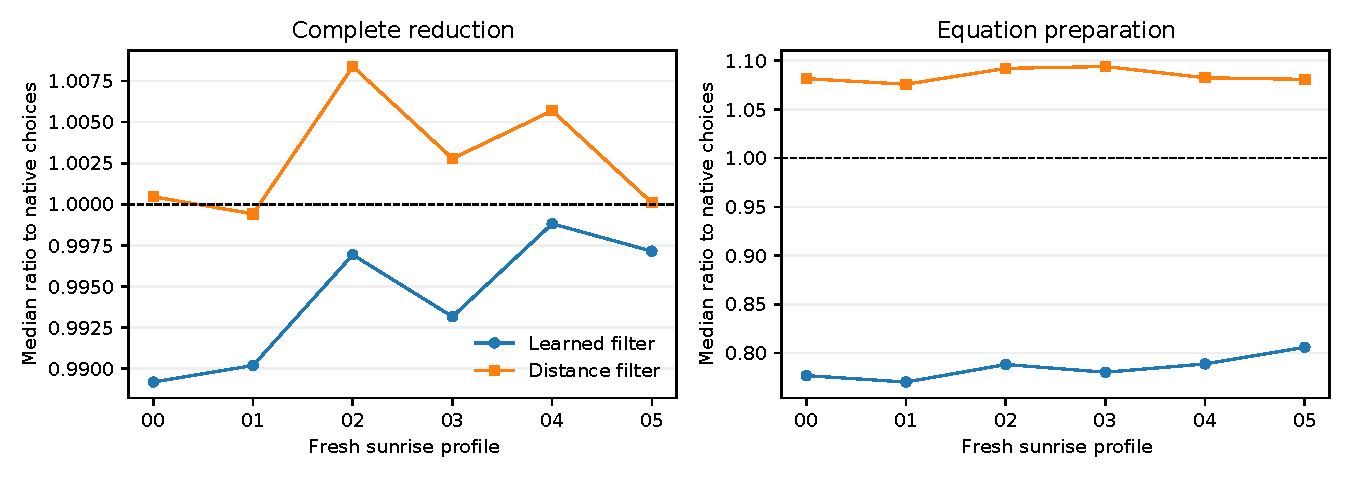
\includegraphics[width=\textwidth]{figures/equation_confirmed_costs.pdf}
 \caption{Fresh confirmation of the restricted sunrise deployment.
 Each profile uses nine repetitions for each method. Complete and
 preparation times include prediction and fallback costs.}
 \label{fig:equation-confirmed}
\end{figure}
The application interface enables this equation policy when it runs with native seed and row choices. Requests for either earlier learned policy retain native equation choices. This guard avoids the slower measured three-model combination.
The broader initial route and its slower vacuum results remain available
as experimental evidence. The measured domain contains two-loop sunrise
integrals with the stated target set, and extension to other target sets
or topologies requires further independent evidence~\cite{KiraEquationSelectionData}.
\FloatBarrier
